%%%%%%%%%%%%%%%%%%%%%%%%%%%%%%%%%%%%%%%%%%%%%%%%%%%%%%%%%%%%%%%%%%%%%%%%%%
%%%%%                         CHAPITRE 1                            %%%%%%
%%%%%%%%%%%%%%%%%%%%%%%%%%%%%%%%%%%%%%%%%%%%%%%%%%%%%%%%%%%%%%%%%%%%%%%%%%

\lhead[\fancyplain{}{\leftmark}]%Pour les pages paires \bfseries
      {\fancyplain{}{}} %Pour les pages impaires
\chead[\fancyplain{}{}]%
      {\fancyplain{}{}}
\rhead[\fancyplain{}{}]%Pour les pages paires 
      {\fancyplain{}{\rightmark}}%Pour les pages impaires \bfseries
\lfoot[\fancyplain{}{}]%
      {\fancyplain{}{}}
\cfoot[\fancyplain{}{\thepage}]%\bfseries
      {\fancyplain{}{\thepage}} %\bfseries
\rfoot[\fancyplain{}{}]%
     {\fancyplain{}{\scriptsize}}


%%%%%%%%%%%%%%%%%%%%%%%%%%%%%%%%%%%%%%%%%%%%%%%%%%%%%%%%%%%%%%%%%%%%%%%%%%
%%%%%                      Start part here                          %%%%%%
%%%%%%%%%%%%%%%%%%%%%%%%%%%%%%%%%%%%%%%%%%%%%%%%%%%%%%%%%%%%%%%%%%%%%%%%%%

\chapter{State of the art}
\label{ch:1}

%======================================================	Résumé du chapitre

\begin{center}
\rule{0.7\linewidth}{.5pt}
\begin{minipage}{0.7\linewidth}
\smallskip

\textit{Résumé du chapitre possible ici.\newline \newline
This chapter is an up-to-date version of the introduction of the previously published paper "Pose2Sim: An End-to-End Workflow for 3D Markerless Sports Kinematics—Part 1: Robustness" \cite{Pagnon_2021} }

%\smallskip
\end{minipage}
\smallskip
\rule{0.7\linewidth}{.5pt}
\end{center}

\minitoc
\newpage



\section{Overall context of kinematics in sports}

Kinematic analysis in sports is a difficult challenge which highlights the limits of classic marker-based methods [1]. Reflective marker-based camera systems are com-plex to set up, require specific lightning conditions, and are overall challenging to use out of a lab. Markers may fall off the body due to sharp accelerations or sweat, as well as hinder the natural movement of athletes, which is likely to affect their warm-up and focus. While the accuracy of landmark location is claimed to be sub-millimetric in marker-based methods [2], marker placement is tedious, intrusive, prone to positioning variability from the operator [3], and subject to skin movement artifacts, especially on soft tissues. Della Croce et al. found out that inter-operator variations in marker placements range from 13 to 25 mm, which can propagate up to 10° in joint angle pre-diction [4,5].  Tissue artifacts account for up to a 2.5 cm marker displacement at the thigh for example, which can cause as much as a 3° error in knee joint angles tissues [6,7]. Joint positions must be calculated explicitly in marker-based methods, which in-troduces more variability: these errors range up to 5 cm, which can contribute up to 3° of error in lower limb joint kinematics [8]. Nevertheless, since marker-based methods benefit from decades of research, they are still considered as the reference method for motion capture.

Consequently, other approaches based on alternative technologies have been in-vestigated over the past years. For example, wearable Inertial Measurement Units (IMUs) offer the advantage of getting away from all camera-related issues such as field of view, occlusions, and controlled environment [9]. They still have the disadvantage of being an external equipment to still wear, involving high technical skills, and being sensitive to ferromagnetic disturbances and exposed to drift over time [10]. Another approach involves depth-field cameras (RGBD), which give access to a 2.5D world (on-ly the depth of the front facing plane of view is measured), or even to full 3D with a network of few RGBD cameras [11–13]. On the other hand, these cameras suffer from a sensitivity to lightning conditions, they work at lower framerates, and they are short-range [14]. 

A recent breakthrough has come from Computer Vision. The explosion of deep-learning based methods from 2D camera videos, for which the research has skyrocket-ed around 2016 [15], is related to the increase in storage capacities and huge improve-ments in GPU computing. A search on ScienceDirect for “deep learning 3D human pose estimation” produced fewer than 100 papers per year until 2015, and the number is now reaching almost 750 over the span of 5 years, fitting an exponential curve (Figure~\ref{fig_exp}).

\begin{figure}[hbtp]
	\centering
	\def\svgwidth{1\columnwidth}
	\fontsize{10pt}{10pt}\selectfont
	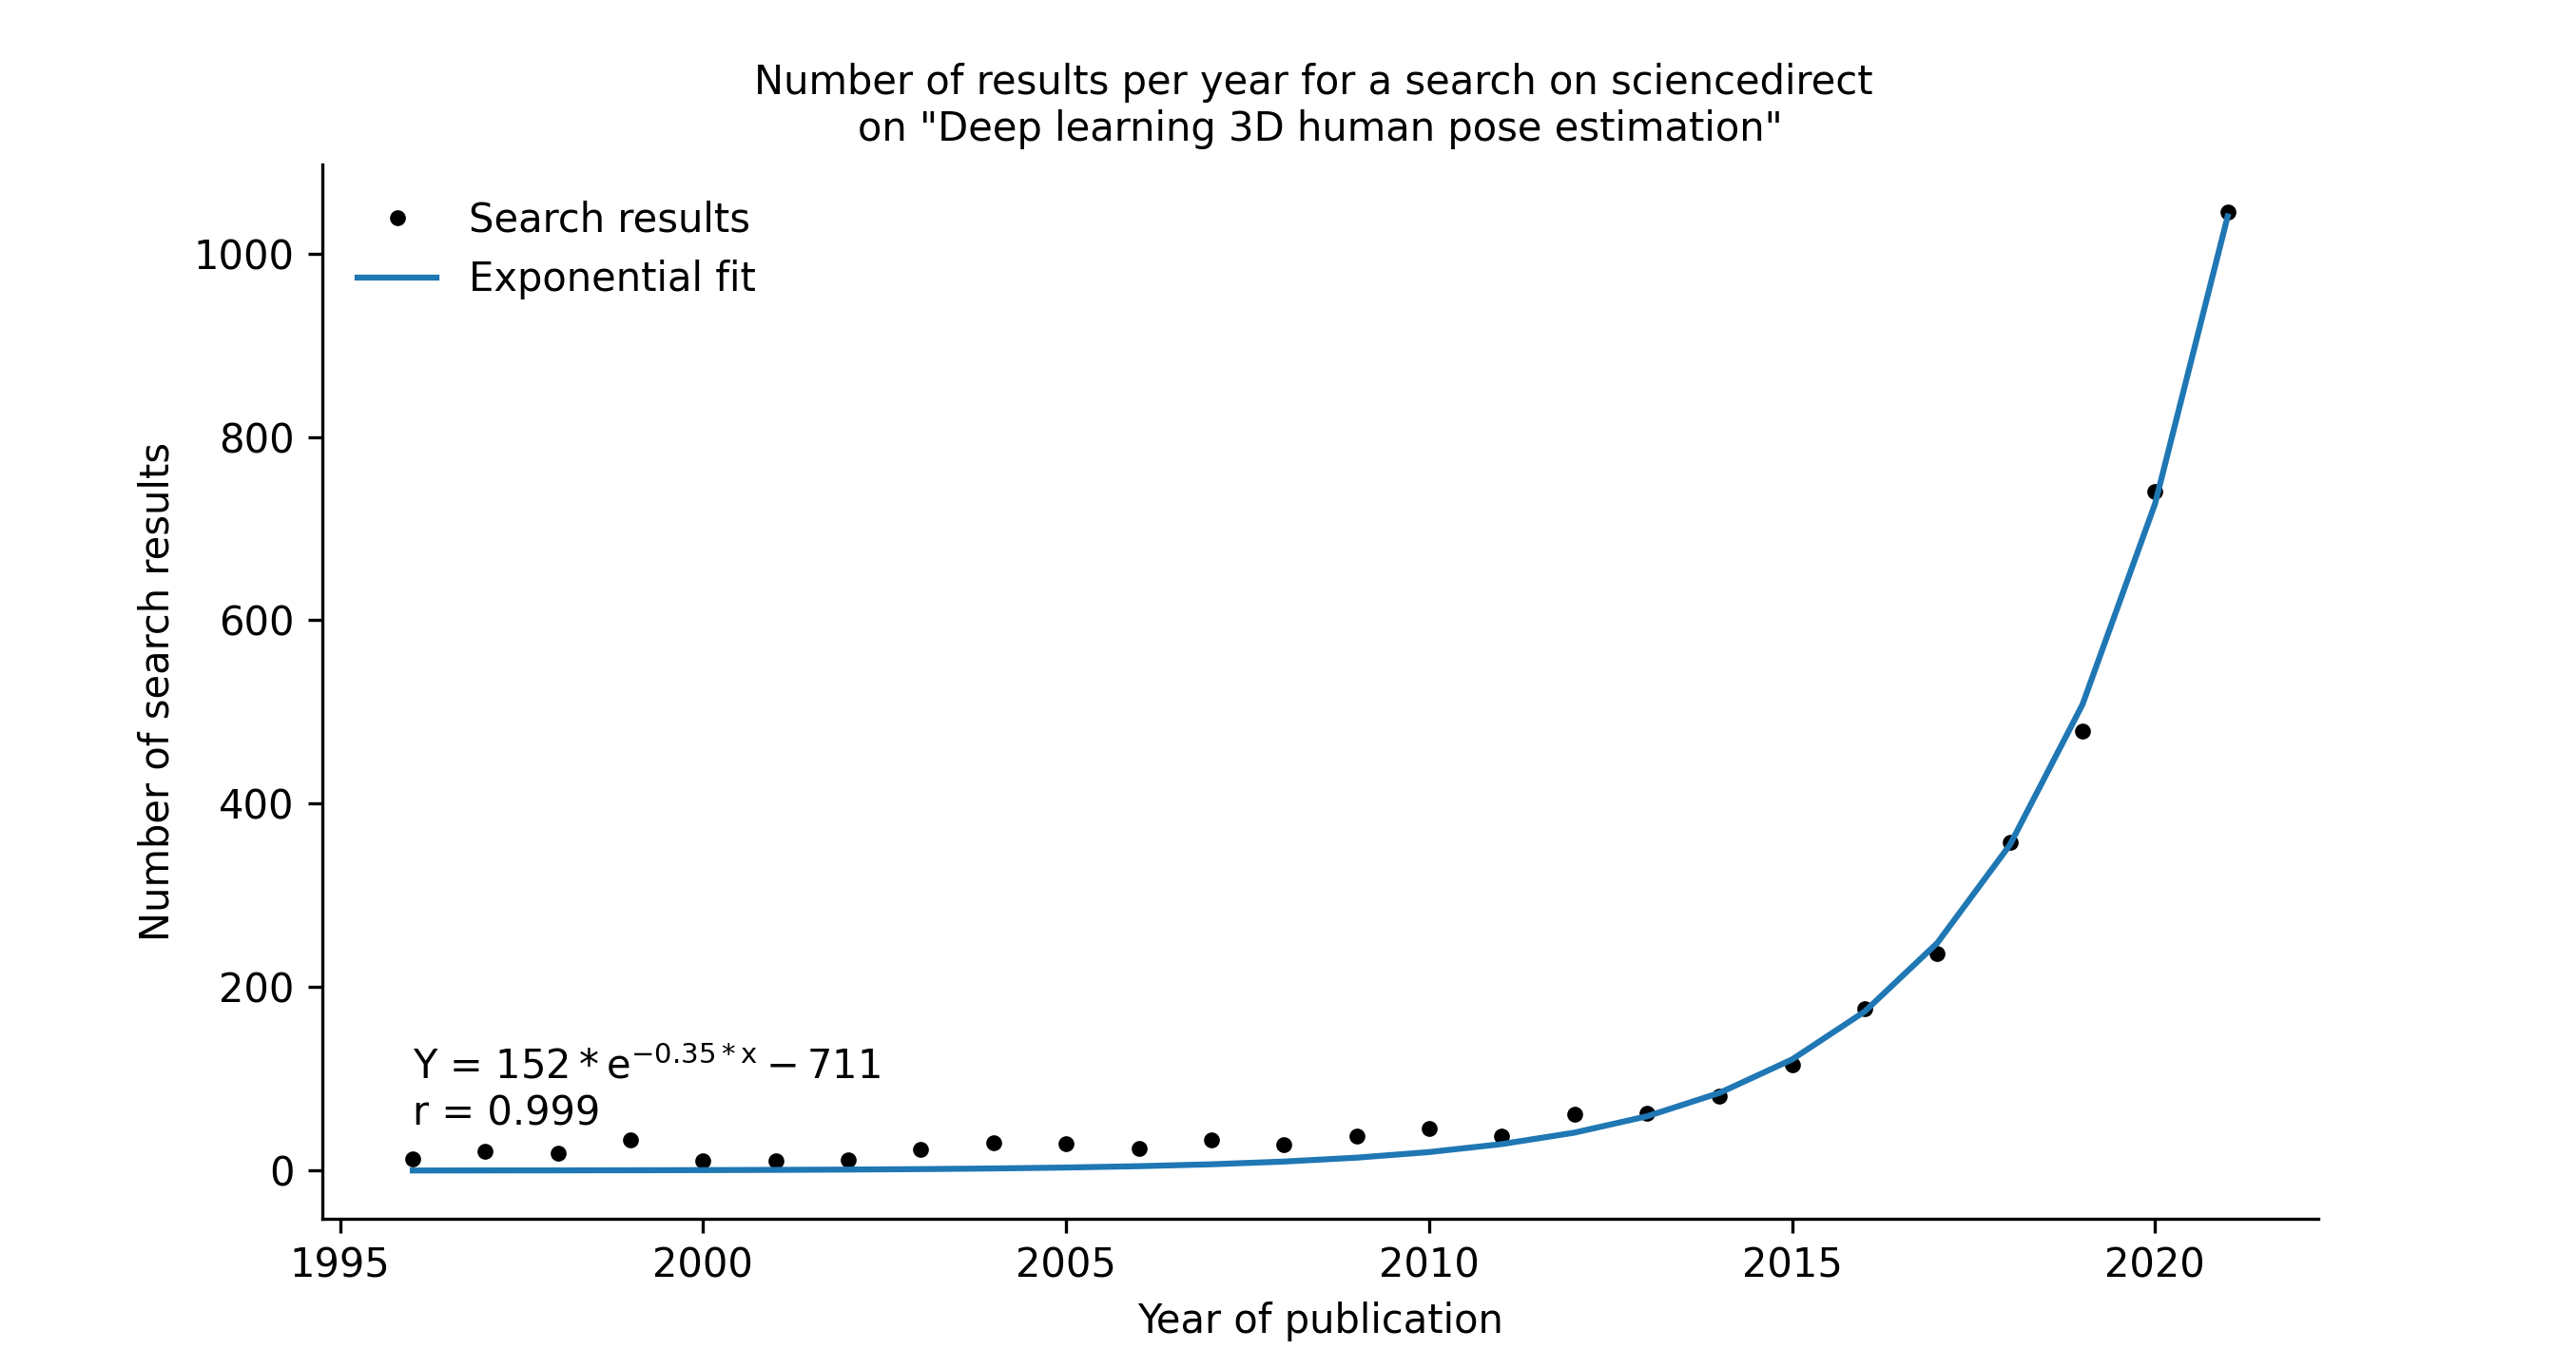
\includegraphics[width=\linewidth]{"../Chap1/Figure/Fig_exp.png"}
	\caption{The search for “deep learning 3D human pose estimation” (dots) fits an exponential curve (line). The search produced less than 100 results until 2015. Over the course of 5 years, the number has reached almost 750 of them, and is now well over a 1000 per year.}
	\label{fig_exp}
\end{figure}

It has rekindled interest from the Biomechanics community towards image-based kinematics, which is where it all started with the invention of chronophotograph in the 19th century by Marey in France, and Muybridge in the USA [16]. Currently, two ap-proaches coexist in human and animal motion analysis for pose estimation: on the one hand, computer vision using deep-learning techniques mostly focus on joint positions only; while the interest of biomechanics lies in kinematics, that involves joint angles. One of the main challenges is to bridge the gap between these two worlds, and to take advantage of deep-learning technologies for kinematic analysis [17,18]. 


\section{2 dimensional analysis}

\subsection{2D pose estimation}
\blindtext

\subsection{2D kinematics from 2D pose estimation}
\blindtext


\section{3 dimensional analysis}

\subsection{3D pose estimation}
\blindtext

\subsection{3D kinematics from 3D pose estimation}
\blindtext


\section{Statement of need}
\blindtext


\section{Exemples}
\subsection{Références}

Exemple de citation \cite{Mündermann2006evolution}, ou là \cite{Collomb2018b}, ou ici \cite{Collomb2018a,Collomb2017a,Collomb2018}. \\


\FloatBarrier
\subsection{Figures}

La Figure~\ref{figure_multiple} est un exemple d'intégration d'une figure multiple. \\
Il est bien entendu possible de faire référence à la Figure~\ref{figure_subplot} ou à la Figure~\ref{figure_polaire}.

\begin{figure}[hbtp]
	\centering
	\begin{subfigure}[b]{0.8\textwidth}
		\centering
		\def\svgwidth{\columnwidth}
		\fontsize{10pt}{10pt}\selectfont\input{../Chap1/Figure/Figure_2.pdf_tex}
		\caption{Exemple subplot} 
		\label{figure_subplot}
	\end{subfigure}
	\qquad
	\begin{subfigure}[b]{0.7\textwidth}
		\centering
		\def\svgwidth{\columnwidth}
		\fontsize{10pt}{10pt}\selectfont\input{../Chap1/Figure/Figure_3.pdf_tex}
		\caption{Exemple diagramme polaire} 
		\label{figure_polaire}
	\end{subfigure}
	\caption{Exemple de Figures multiple} 
	\label{figure_multiple}
\end{figure}



\FloatBarrier
\subsection{Tableaux}

Générateur en ligne \href{http://www.tablesgenerator.com/latex_tables}{ici}. \\

Un exemple de tableau générée par cet outil est présenté Table~\ref{tableau_exemple}.

\begin{table}[]
\centering
\begin{tabular}{c|c|c|c|}
\cline{2-4}
                               & \textbf{A}                 & \textbf{B} & \textbf{C} \\ \hline
\multicolumn{1}{|c|}{$\alpha$} & \multicolumn{3}{c|}{\textit{fusion}}                 \\ \hline
\multicolumn{1}{|c|}{$\beta$}  & \multirow{2}{*}{\textit{}} & \textit{1} & \textit{2} \\ \cline{1-1} \cline{3-4} 
\multicolumn{1}{|c|}{$\Delta$} &                            & \textit{3} & \textit{4} \\ \hline
\end{tabular}
\caption{Exemple de tableau}
\label{tableau_exemple}
\end{table}


\FloatBarrier
\section{Section 2}
\subsection{Sous-section 1}
\blindtext

\subsection{Sous-section 2}
\blindtext